\chapter{Validated Results}
\label{cha:results}

To demonstrate the geo-based media player, we went out and did some recordings to test the functionalities we designed and implemented in this thesis. We went to “Blåa havet” in front of Kårallen, located at Linköping University, where some students were promoting an upcoming event with some activities. We found that this was a suitable point of interest to record from different angles for our testing case. As we only had two cameras available at the time we made three sets of recordings consisting of two recordings each, with each set displaying the same scene from two different locations and angles at the same time. The desired outcomes of this test was to prove the accuracy of the relative placement algorithm and, within the interface, be able to swap between the recordings to view the same object at one point in time from different angles.

\section{Position Algorithm}
\label{sec:positionalgorithm}

To demonstrate the accuracy of the relative placement of geographical points in the interface, we noted the GPS-coordinates and angles at the used recording locations. We then input the coordinates into Google Maps as seen in Figure \ref{fig:googlemaps}, which is used here as a reference to prove the accuracy of our placement algorithm. We also input the same latitude and longitude values into our interface along with the angles used in the recordings to test our algorithm for a few objects. We later input another larger set of coordinates into the interface including many objects to load test the algorithm. Figure \ref{fig:GeomapVsGoogleLessThan10objects} shows the comparison between the algorithm's object placement and the Google Maps reference with the coordinates used in the test case and Figure \ref{fig:GeomapVsGoogleMoreThan10objects} shows a similar comparison in the algorithm's load test. In these figures the displayed yellow stars represents Google Maps' placement of the given coordinates while the arrow-dots represents the same respective placement of the coordinates as received from the interface.


\begin{figure}[ht!]
\begin{center}
	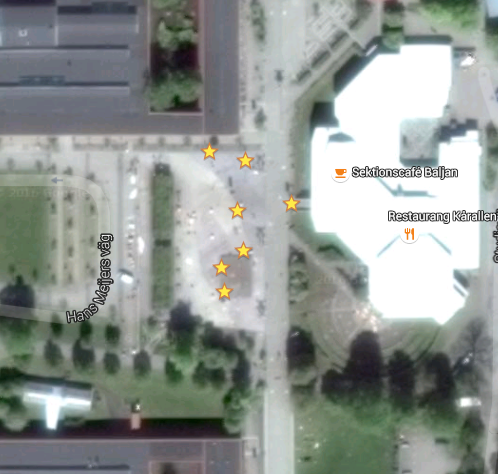
\includegraphics[scale=0.64]{Google_Maps.png}
	\caption{Google Maps view of the Streaming locations}
	\label{fig:googlemaps}
\end{center}
\end{figure}

\begin{figure}
\begin{subfigure}[b]{0.5\textwidth}
        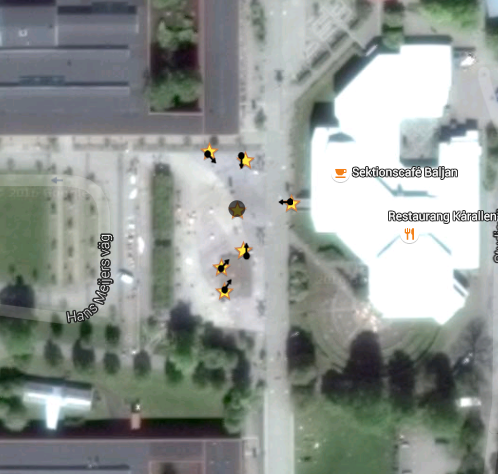
\includegraphics[width=\textwidth]{GeomapVsGooglemindrean10.png}
        \caption{Geo-map compared to google map with less than 10 objects}
        \label{fig:GeomapVsGoogleLessThan10objects}
    \end{subfigure}\hfill 
    \hspace{3px}
    \begin{subfigure}[b]{0.51\textwidth}
        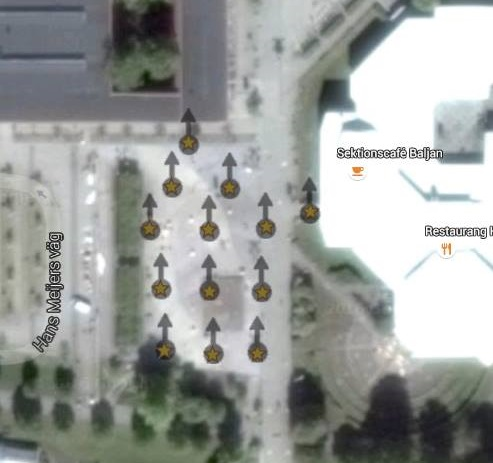
\includegraphics[width=\textwidth]{GeomapVsGooglefleran10.png}
        \caption{Geo-map compared to google map with more than 10 objects}
        \label{fig:tiger}
    \label{fig:GeomapVsGoogleMoreThan10objects}
    \end{subfigure}
	\caption{Geo-map compared to google map using equirectangular algorithm}
	\label{fig:GeomapVsGoogleWithLessThan10objects}
\end{figure}

The placement of the arrow points in Figure \ref{fig:GeomapVsGoogleLessThan10objects} is almost an exact match to the Google Maps reference stars for the respective coordinates, at least in terms off relativity. There is a slight difference between interface's placement and the reference in this figure and the reason for this is that our method for rotating the arrow points is not optimal. The default and only way of rotating a graphical object provided by our programming tools is to rotate the object around its top-left corner. Due to this we added some functionality to this existing rotation function to make the objects rotate around its center instead. Because this rotation code is not optimal there is a very slight deviation from its supposed placement. With the load test however, we did not angle the arrow points as shown in Figure \ref{fig:GeomapVsGoogleMoreThan10objects}. Because the suboptimal rotation function does not take place here the algorithm's relative placement is exactly on point with its reference.

This would prove the accuracy of our relative placement of the geographical points, albeit with a slightly better precision if the objects are not rotated. The rotation function will be further discussed in \textit{Chapter \ref{cha:discussion}}.

\section{Geo-based Streaming}
\label{sec:geobasedstreaming}

As we have mentioned before our implementations is as shown in Figure \ref{fig:gpsinterface}, where we have a button that opens the geographical map, a circle that represents a “map” and arrows pointing in a direction that represents streamers and videos. When a video is selected the arrow is highlighted and that video is then played. In our test case, we set up two cameras at a time and did recordings of 90 seconds each. In these videos we captured many people doing various activities. There were people jumping the trampoline, using hoverboards, walking and biking around. When we input these three sets of two recordings each into our media player, we could swap between the two recordings of each set and watch these same events unfold from different positions and angles. In Figures \ref{fig:testview1A} and \ref{fig:testview2A} two different recordings are selected and they show the same event where, for example, the guy inside the red circle in the pictures are hoverboarding in front of the red shirt guy the same time of the videos. If we look at Figures \ref{fig:testview1B} and \ref{fig:testview2B} they show the geo-map interface of the views. Both interfaces shows that a different stream object is highlighted when a different view is shown. This would prove the desired functionality of where the user can display the same events unfold from different geographical positions and angles.

\begin{figure}
\begin{subfigure}[b]{0.5\textwidth}
 	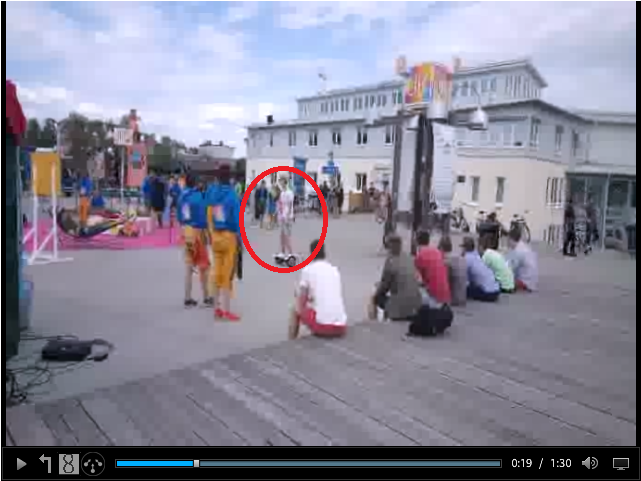
\includegraphics[width=\linewidth]{Hoverboard_1.png}
  	\caption{Test view 1 without the interface visible}\label{fig:testview1A}
    \end{subfigure}\hfill 
    \hspace{3px}
    \begin{subfigure}[b]{0.5\textwidth}
	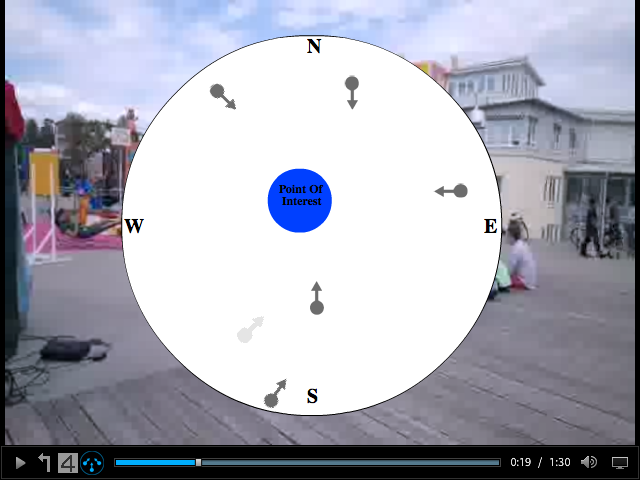
\includegraphics[width=\linewidth]{Hoverboard1medmap.png}
  	\caption{Test view 1 with the interface visible}\label{fig:testview1B}
    \end{subfigure}
	\caption{Test view 1}
	\label{fig:testview1}
\end{figure}

\begin{figure}
\begin{subfigure}[b]{0.5\textwidth}
 	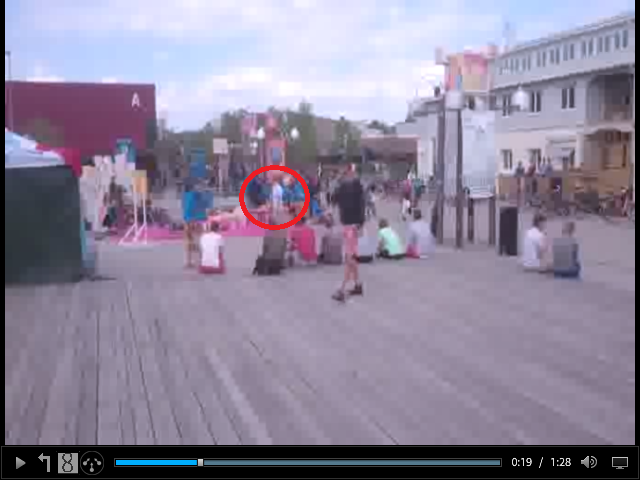
\includegraphics[width=\linewidth]{Hoverboard_2.png}
  	\caption{Test view 2 without the interface visible}\label{fig:testview2A}
    \end{subfigure}\hfill 
    \hspace{3px}
    \begin{subfigure}[b]{0.5\textwidth}
	 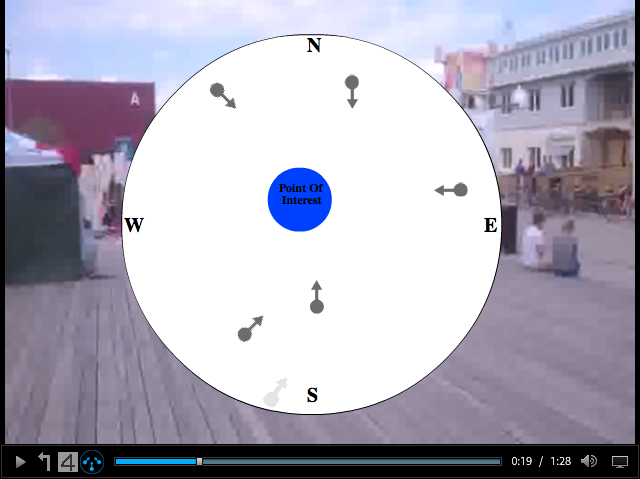
\includegraphics[width=\linewidth]{Hoverboard2medmap.png}
 	\caption{Test view 2 with the interface visible}\label{fig:testview2B}
    \end{subfigure}
	\caption{Test view 2}
	\label{fig:testview2}
\end{figure}

\section{Consistency with On-demand Switching}
Even though prefetching is not implemented we can still test the consistency of the on-demand switching, looking at the time it takes to switch between different videos on-demand. This test was done by clicking between different stream objects on interface and tracking the time it takes to load a video to the media player. Switching between different videos was done 200 times and two graphical representations of how long time each video switch took is shown in Figures \ref{fig:histogram} and \ref{fig:cdf}. The histogram in Figure \ref{fig:histogram} represents the frequency for a video switch in a certain time interval and the Cumulative Distribution Function (CDF) in Figure \ref{fig:cdf} shows the probability that a certain time \textit{x} will occur. We can see from the CDF graph that the probability that a video switch take less than 140 milliseconds is around 70 $\%$ and that the probability for a video switch under 160 milliseconds is around 90 $\%$. This means that a video switch will unlikely take more than 160 milliseconds or even more than 200 milliseconds. The average time it took to switch is roughly 140 milliseconds, or 137 milliseconds to be precise. The median is 129 milliseconds and the standard deviation is around 28 $\%$.

The times for switching is likely a bit faster than shown because of how checking the time is done. The time starts when the object is clicked and a new advertisement is created. After that a new media player is created and the the URL will be retrieved through the AMS 5. The URL will then be sent to the plug-in script and then called by the \textit{AdvertisementPluginInfo} class. The URL is then prebuffered a little bit before the video is ready to be played in which the timer will stop. If prebuffering of the video can be done in a more efficient way with optimized prefetching similiar to what is done in the project \cite{optimizedstreaming} the time would likely have been a bit faster.

This test is done from another computer which did not host AMS 5 which means that it had to send requests of the streams to the computer hosting the AMS 5 in order to receive the videos. Keep in mind if this consistency test were done on a different performing setup with another set of computers and connections, this result would likely vary.

\newpage

\begin{figure}[ht!]
\begin{center}
	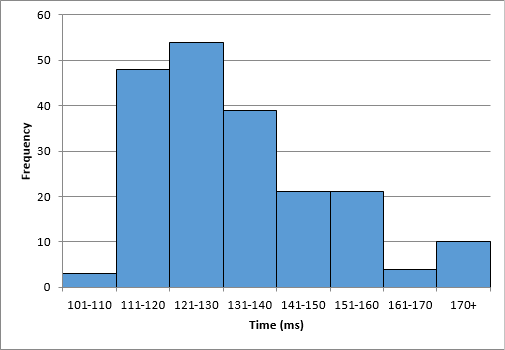
\includegraphics[scale=1]{histogram.png}
	\caption{Histogram with the click-time interval}
	\label{fig:histogram}
\end{center}
\end{figure}

\begin{figure}[ht!]
\begin{center}
	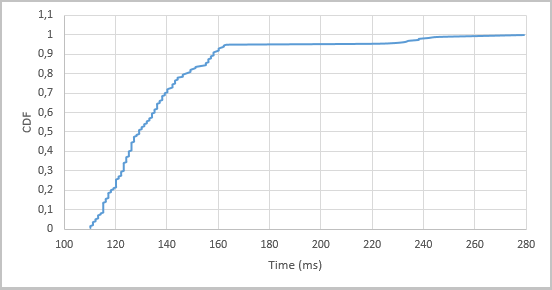
\includegraphics[scale=1]{CDF.png}
	\caption{CDF with the click-time interval}
	\label{fig:cdf}
\end{center}
\end{figure}